\gdef\problemNumber{GT R-13.15 (modified)}
\def\problemText{
How many biconnected components would be in the graph shown in Figure~$13.5$a
if we were to remove the edge $(B,C)$ and the edge $(N,K)$? List the edges in
each biconnected component.\\[12pt]
}
\def\problemSolution{
\textcolor{blue}{
\textbf{Answer:}\\[6pt]
Answer goes here
Note: Here is the graph with the two edges removed:\\
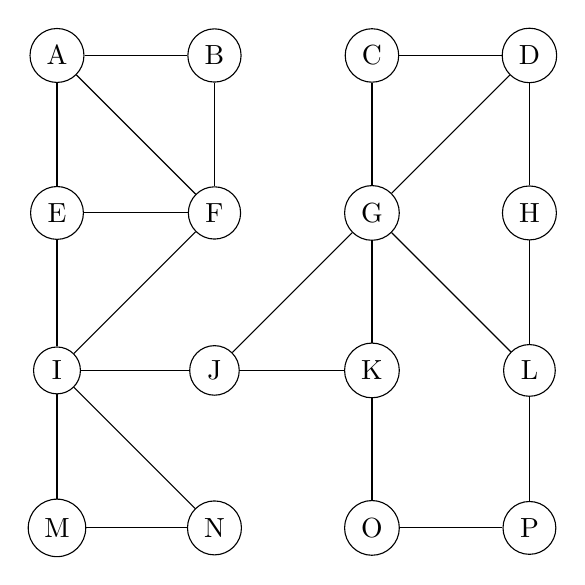
\begin{tikzpicture}
    \node[circle,draw] at (0,6) (a) {A};
    \node[circle,draw] at (2,6) (b) {B};
    \node[circle,draw] at (4,6) (c) {C};
    \node[circle,draw] at (6,6) (d) {D};
    \node[circle,draw] at (0,4) (e) {E};
    \node[circle,draw] at (2,4) (f) {F};
    \node[circle,draw] at (4,4) (g) {G};
    \node[circle,draw] at (6,4) (h) {H};
    \node[circle,draw] at (0,2) (i) {I};
    \node[circle,draw] at (2,2) (j) {J};
    \node[circle,draw] at (4,2) (k) {K};
    \node[circle,draw] at (6,2) (l) {L};
    \node[circle,draw] at (0,0) (m) {M};
    \node[circle,draw] at (2,0) (n) {N};
    \node[circle,draw] at (4,0) (o) {O};
    \node[circle,draw] at (6,0) (p) {P};
    \draw[-] (a) -- (b);
    \draw[-] (a) -- (e);
    \draw[-] (a) -- (f);
    \draw[-] (b) -- (f);
    \draw[-] (c) -- (d);
    \draw[-] (c) -- (g);
    \draw[-] (d) -- (g);
    \draw[-] (d) -- (h);
    \draw[-] (e) -- (f);
    \draw[-] (e) -- (i);
    \draw[-] (f) -- (i);
    \draw[-] (g) -- (j);
    \draw[-] (g) -- (k);
    \draw[-] (g) -- (l);
    \draw[-] (h) -- (l);
    \draw[-] (i) -- (j);
    \draw[-] (i) -- (m);
    \draw[-] (i) -- (n);
    \draw[-] (j) -- (k);
    \draw[-] (k) -- (o);
    \draw[-] (l) -- (p);
    \draw[-] (m) -- (n);
    \draw[-] (o) -- (p);
\end{tikzpicture}
}
}
\gdef\problemOutcomes{CS 2, CS 6, 5870-2}
